\begin{enumerate}[label=\thesubsection.\arabic*, ref=\thesubsection.\theenumi]
\item 
Find :
\begin{align*}
	\int \frac{\sin^2 x - \cos^2 x}{\sin x \cos x}\, dx
\end{align*}
\hfill (CBSE~2017)
\\
\solution
Splitting the numerator,
\begin{align}
	\frac{\sin^2 x - \cos^2 x}{\sin x\cos x} = \frac{\sin x}{\cos x} - \frac{\cos x}{\sin x} = \tan x - \cot x
\end{align}
From \eqref{eq:EE26BTECH11229-int-tancot},
\begin{align}
	\int \brak{\tan x - \cot x}\, dx &= -\ln\abs{\cos x} - \ln\abs{\sin x} + C
	\\
	&= -\ln\abs{\sin x\cos x} + C
\end{align}
Since $\sin x\cos x = \frac{1}{2}\sin 2x$, this is also $-\ln\abs{\sin 2x} + C^{\prime}$.
\item 
Find the distance between the planes $2x - y + 2z = 5$ and $5x - 2.5y + 5z = 20$.
\hfill (CBSE~2017)
\\
\solution
The first plane is, from \eqref{eq:EE26BTECH11229-normal-form},
\begin{align}
	\myvec{2 & -1 & 2}\vec{x} = 5
\end{align}
Dividing the second equation by $2.5$,
\begin{align}
	\myvec{5 & -2.5 & 5}\vec{x} = 20 \implies \myvec{2 & -1 & 2}\vec{x} = 8
\end{align}
The planes are parallel with
\begin{align}
	\vec{n} = \myvec{2 \\ -1 \\ 2}, \quad c_1 = 5, \quad c_2 = 8, \quad \norm{\vec{n}} = \sqrt{4 + 1 + 4} = 3
\end{align}
From \eqref{eq:EE26BTECH11229-plane-dist},
\begin{align}
	d = \frac{\abs{8 - 5}}{3} = 1
\end{align}

The following code verifies the solution
\begin{lstlisting}[frame=single, basicstyle=\rmfamily, escapeinside={(*@}{@*)}]
(*@\makebox[\dimexpr\linewidth-2\fboxsep-2\fboxrule\relax][c]{codes/distance.py}@*)
\end{lstlisting}

\item 
If for any $2 \times 2$ square matrix $\vec{A}$, $\vec{A}\,\text{adj}\brak{\vec{A}} = \myvec{8 & 0 \\ 0 & 8}$, then write the value of $\mydet{\vec{A}}$.
\hfill (CBSE~2017)
\\
\solution
From \eqref{eq:EE26BTECH11229-adj},
\begin{align}
	\vec{A}\,\text{adj}\brak{\vec{A}} = \mydet{\vec{A}}\vec{I} = \myvec{8 & 0 \\ 0 & 8} = 8\vec{I}
\end{align}
Comparing the entries,
\begin{align}
	\mydet{\vec{A}} = 8
\end{align}
As a check, taking the trace of both sides using \eqref{eq:EE26BTECH11229-trace},
\begin{align}
	\text{tr}\brak{\mydet{\vec{A}}\vec{I}} = 2\mydet{\vec{A}} = \text{tr}\brak{8\vec{I}} = 16 \implies \mydet{\vec{A}} = 8
\end{align}

The following code verifies the solution
\begin{lstlisting}[frame=single, basicstyle=\rmfamily, escapeinside={(*@}{@*)}]
(*@\makebox[\dimexpr\linewidth-2\fboxsep-2\fboxrule\relax][c]{codes/determinant.py}@*)
\end{lstlisting}
\item 
A die, whose faces are marked 1, 2, 3 in red and 4, 5, 6 in green, is tossed. Let $A$ be the event ``number obtained is even'' and $B$ be the event ``number obtained is red''. Find if $A$ and $B$ are independent events.
\hfill (CBSE~2017)
\\
\solution
The events are
\begin{align}
	A = \cbrak{2, 4, 6}, \quad B = \cbrak{1, 2, 3}, \quad AB = \cbrak{2}
\end{align}
From \eqref{eq:EE26BTECH11229-die-pmf} and \eqref{eq:EE26BTECH11229-event-pmf},
\begin{align}
	\pr{A} = \frac{3}{6} = \frac{1}{2}, \quad \pr{B} = \frac{3}{6} = \frac{1}{2}, \quad \pr{AB} = \frac{1}{6}
\end{align}
From \eqref{eq:EE26BTECH11229-indep}, 
\begin{align}
	\pr{A}\pr{B} = \frac{1}{4} \neq \frac{1}{6} = \pr{AB}
\end{align}
Therefore, $A$ and $B$ are not independent events.

The following code verifies the solution
\begin{lstlisting}[frame=single, basicstyle=\rmfamily, escapeinside={(*@}{@*)}]
(*@\makebox[\dimexpr\linewidth-2\fboxsep-2\fboxrule\relax][c]{codes/dice.c}@*)
\end{lstlisting}
\item 
Two tailors, $A$ and $B$, earn \rupee~300 and \rupee~400 per day respectively. $A$ can stitch 6 shirts and 4 pairs of trousers while $B$ can stitch 10 shirts and 4 pairs of trousers per day. To find how many days should each of them work and if it is desired to produce at least 60 shirts and 32 pairs of trousers at a minimum labour cost, formulate this as an LPP.
\hfill (CBSE~2017)
\\
\solution
Let $A$ work for $x$ days and $B$ work for $y$ days. The labour cost is
\begin{align}
	Z = 300x + 400y
\end{align}
The number of shirts and trousers stitched should be at least $60$ and $32$ respectively,
\begin{align}
	6x + 10y &\ge 60
	\\
	4x + 4y &\ge 32
\end{align}
and the number of days cannot be negative, $x \ge 0$, $y \ge 0$. From \eqref{eq:EE26BTECH11229-lpp}, the LPP is
\begin{align}
	\text{minimise } Z = \myvec{300 & 400}\myvec{x \\ y} \quad \text{subject to } \myvec{6 & 10 \\ 4 & 4}\myvec{x \\ y} \succeq \myvec{60 \\ 32}, \ \myvec{x \\ y} \succeq \vec{0}
\end{align}
Equivalently, 
\begin{align}
	\text{minimise } Z = 300x + 400y \quad \text{subject to } 3x + 5y \ge 30, \ x + y \ge 8, \ x, y \ge 0
\end{align}
To find the number of days, the lines $3x + 5y = 30$ and $x + y = 8$ meet at the point given by
\begin{align}
	\myvec{3 & 5 \\ 1 & 1}\myvec{x \\ y} = \myvec{30 \\ 8}
	\implies x = 5, \quad y = 3
\end{align}
The feasible region is unbounded, with the corner points
\begin{align}
	\brak{0, 8}, \quad \brak{5, 3}, \quad \brak{10, 0}
\end{align}
where $\brak{0, 8}$ and $\brak{10, 0}$ are the points where the lines $x + y = 8$ and $3x + 5y = 30$ meet the $y$-axis and the $x$-axis respectively, and each of them satisfies the other constraint. From \eqref{eq:EE26BTECH11229-corner}, evaluating $Z$ at the corner points,
\begin{align}
	Z\brak{0, 8} &= 400\brak{8} = 3200
	\\
	Z\brak{5, 3} &= 300\brak{5} + 400\brak{3} = 2700
	\\
	Z\brak{10, 0} &= 300\brak{10} = 3000
\end{align}
Since the region is unbounded, we check that $2700$ is the true minimum. For every feasible point,
\begin{align}
	Z = 50\brak{3x + 5y} + 150\brak{x + y} \ge 50\brak{30} + 150\brak{8} = 2700
\end{align}
so no feasible point gives a smaller cost. Therefore, $A$ should work for $5$ days and $B$ for $3$ days, and the minimum labour cost is \rupee~2700. As a check, $6\brak{5} + 10\brak{3} = 60$ shirts and $4\brak{5} + 4\brak{3} = 32$ pairs of trousers are produced.

The following code verifies the solution
\begin{lstlisting}[frame=single, basicstyle=\rmfamily, escapeinside={(*@}{@*)}]
(*@\makebox[\dimexpr\linewidth-2\fboxsep-2\fboxrule\relax][c]{codes/tailor\_cost.py}@*)
\end{lstlisting}
\item 
Find :
\begin{align*}
	\int \frac{dx}{5 - 8x - x^2}
\end{align*}
\hfill (CBSE~2017)
\\
\solution
Completing the square,
\begin{align}
	5 - 8x - x^2 = 21 - \brak{x^2 + 8x + 16} = \brak{\sqrt{21}}^2 - \brak{x + 4}^2
\end{align}
Substituting $u = x + 4$, $du = dx$, and using \eqref{eq:EE26BTECH11229-int-a2x2} with $a = \sqrt{21}$,
\begin{align}
	\int \frac{dx}{5 - 8x - x^2} = \int \frac{du}{\brak{\sqrt{21}}^2 - u^2}
	= \frac{1}{2\sqrt{21}}\ln\abs{\frac{\sqrt{21} + u}{\sqrt{21} - u}} + C
\end{align}
yielding
\begin{align}
	\int \frac{dx}{5 - 8x - x^2} = \frac{1}{2\sqrt{21}}\ln\abs{\frac{\sqrt{21} + x + 4}{\sqrt{21} - x - 4}} + C
\end{align}
\item 
Find the value of $c$ in Rolle's theorem for the function $f\brak{x} = x^3 - 3x$ in $\sbrak{-\sqrt{3}, 0}$.
\hfill (CBSE~2017)
\\
\solution
The function $f\brak{x}$ is a polynomial, so it is differentiable, and hence continuous, from \eqref{eq:EE26BTECH11229-diff-cont}. At the end points,
\begin{align}
	f\brak{-\sqrt{3}} = -3\sqrt{3} + 3\sqrt{3} = 0, \quad f\brak{0} = 0
\end{align}
The conditions of \eqref{eq:EE26BTECH11229-rolle} hold, so there exists $c \in \brak{-\sqrt{3}, 0}$ with $f^{\prime}\brak{c} = 0$,
\begin{align}
	f^{\prime}\brak{x} &= 3x^2 - 3 = 3\brak{x - 1}\brak{x + 1} = 0
	\\
	\implies x &= \pm 1
\end{align}
Since $-\sqrt{3} \approx -1.732$, only $x = -1$ lies in $\brak{-\sqrt{3}, 0}$, so
\begin{align}
	c = -1
\end{align}
Using \eqref{eq:EE26BTECH11229-newton} on $f^{\prime}\brak{x}$, with $f^{\prime\prime}\brak{x} = 6x$,
\begin{align}
	x_{n+1} = x_n - \frac{3x_n^2 - 3}{6x_n} = \frac{x_n^2 + 1}{2x_n}
\end{align}
For $x_0 = -1.5$, the iterations are $x_1 \approx -1.0833$, $x_2 \approx -1.0032$, $x_3 \approx -1.0000$, which converge to $c = -1$.
The following code verifies the solution
\begin{lstlisting}[frame=single, basicstyle=\rmfamily, escapeinside={(*@}{@*)}]
(*@\makebox[\dimexpr\linewidth-2\fboxsep-2\fboxrule\relax][c]{codes/rolle.c}@*)
\end{lstlisting}
\item 
Show that the function $f\brak{x} = x^3 - 3x^2 + 6x - 100$ is increasing on $\mathbb{R}$.
\hfill (CBSE~2017)
\\
\solution
Differentiating,
\begin{align}
	f^{\prime}\brak{x} = 3x^2 - 6x + 6 = 3\sbrak{\brak{x - 1}^2 + 1}
\end{align}
Since $\brak{x - 1}^2 \ge 0$ for all $x \in \mathbb{R}$,
\begin{align}
	f^{\prime}\brak{x} \ge 3 > 0
\end{align}
Hence, from \eqref{eq:EE26BTECH11229-increasing}, $f\brak{x}$ is strictly increasing on $\mathbb{R}$.

The following code generates \figref{fig:EE26BTECH11229-increasing}
\begin{lstlisting}[frame=single, basicstyle=\rmfamily, escapeinside={(*@}{@*)}]
(*@\makebox[\dimexpr\linewidth-2\fboxsep-2\fboxrule\relax][c]{codes/Increasing.py}@*)
\end{lstlisting}
\begin{figure}[H]
    \centering
    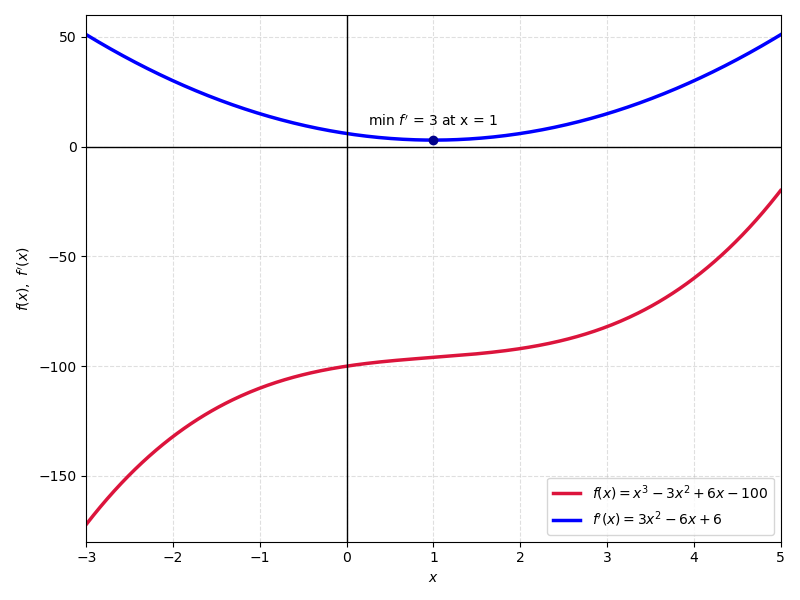
\includegraphics[width=0.75\linewidth]{figs/Increasing.png}
    \caption{Increasing function}
    \label{fig:EE26BTECH11229-increasing}
\end{figure}
\item 
The length $x$, of a rectangle is decreasing at the rate of 5 cm/minute and the width $y$, is increasing at the rate of 4 cm/minute. When $x = 8$ cm and $y = 6$ cm, find the rate of change of the area of the rectangle.
\hfill (CBSE~2017)
\\
\solution
The area is $A = xy$, with
\begin{align}
	\frac{dx}{dt} = -5 \text{ cm/min}, \quad \frac{dy}{dt} = 4 \text{ cm/min}
\end{align}
From \eqref{eq:EE26BTECH11229-rate}, at $x = 8$, $y = 6$,
\begin{align}
	\frac{dA}{dt} = 8\brak{4} + 6\brak{-5} = 32 - 30 = 2 \text{ cm}^2\text{/min}
\end{align}
The area is increasing at the rate of $2 \text{ cm}^2\text{/min}$.
The following code verifies the solution
\begin{lstlisting}[frame=single, basicstyle=\rmfamily, escapeinside={(*@}{@*)}]
(*@\makebox[\dimexpr\linewidth-2\fboxsep-2\fboxrule\relax][c]{codes/area.c}@*)
\end{lstlisting}
\item 
Evaluate :
\begin{align*}
	\int_{0}^{\pi} \frac{x\tan x}{\sec x + \tan x}\, dx
\end{align*}
\hfill (CBSE~2017)
\\
\solution
Let
\begin{align}
	I = \int_{0}^{\pi} \frac{x\tan x}{\sec x + \tan x}\, dx
\end{align}
From \eqref{eq:EE26BTECH11229-prop-int} and \eqref{eq:EE26BTECH11229-trig-pi},
\begin{align}
	I = \int_{0}^{\pi} \frac{\brak{\pi - x}\brak{-\tan x}}{-\sec x - \tan x}\, dx
	= \int_{0}^{\pi} \frac{\brak{\pi - x}\tan x}{\sec x + \tan x}\, dx
\end{align}
Adding the two expressions of $I$,
\begin{align}
	2I = \pi\int_{0}^{\pi} \frac{\tan x}{\sec x + \tan x}\, dx
	= \pi\int_{0}^{\pi} \frac{\sin x}{1 + \sin x}\, dx
	= \pi\int_{0}^{\pi} \sbrak{1 - \frac{1}{1 + \sin x}}dx
\end{align}
from \eqref{eq:EE26BTECH11229-trig-id}. Using \eqref{eq:EE26BTECH11229-trig-id} and \eqref{eq:EE26BTECH11229-deriv-sec},
\begin{align}
	\int_{0}^{\pi} \frac{dx}{1 + \sin x} = \int_{0}^{\pi}\brak{\sec^2 x - \sec x\tan x}dx
	= \sbrak{\tan x - \sec x}_{0}^{\pi}
\end{align}
Here $\tan x - \sec x = -\frac{\cos x}{1 + \sin x}$ is continuous on $\sbrak{0, \pi}$, so
\begin{align}
	\sbrak{-\frac{\cos x}{1 + \sin x}}_{0}^{\pi} = 1 - \brak{-1} = 2
\end{align}
Therefore,
\begin{align}
	2I = \pi\brak{\pi - 2}
	\implies I = \frac{\pi\brak{\pi - 2}}{2}
\end{align}

The following code generates \figref{fig:EE26BTECH11229-integral_xtanx}
\begin{lstlisting}[frame=single, basicstyle=\rmfamily, escapeinside={(*@}{@*)}]
(*@\makebox[\dimexpr\linewidth-2\fboxsep-2\fboxrule\relax][c]{codes/Integral\_xtanx.py}@*)
\end{lstlisting}
\begin{figure}[H]
    \centering
    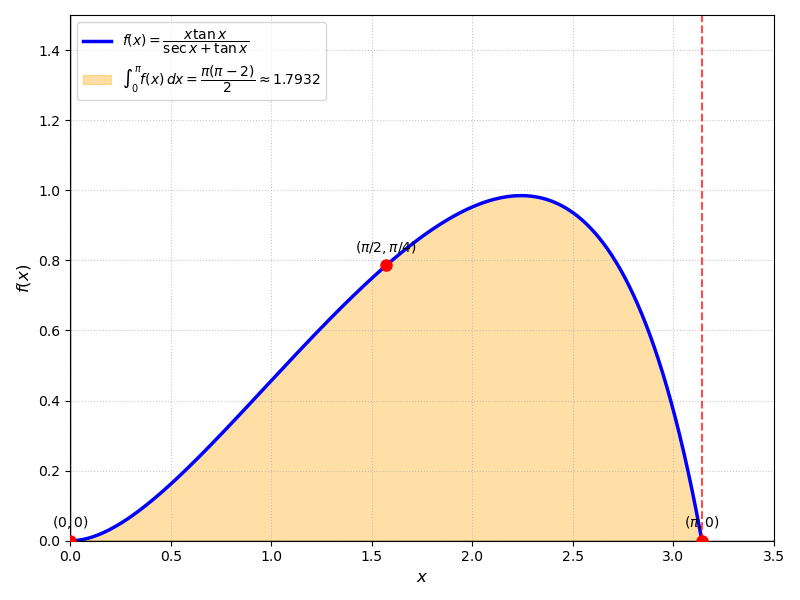
\includegraphics[width=0.75\linewidth]{figs/Integral_xtanx.png}
    \caption{Integral of $x\tan x$}
    \label{fig:EE26BTECH11229-integral_xtanx}
\end{figure}
\item 
Evaluate :
\begin{align*}
	\int_{1}^{4} \cbrak{\abs{x - 1} + \abs{x - 2} + \abs{x - 4}}\, dx
\end{align*}
\hfill (CBSE~2017)
\\
\solution
From \eqref{eq:EE26BTECH11229-abs-def}, for $1 \le x \le 4$, $\abs{x - 1} = x - 1$ and $\abs{x - 4} = 4 - x$, while $\abs{x - 2}$ changes at $x = 2$. Thus the integrand is
\begin{align}
	g\brak{x} = \begin{cases}
		\brak{x - 1} + \brak{2 - x} + \brak{4 - x} = 5 - x, & 1 \le x \le 2
		\\
		\brak{x - 1} + \brak{x - 2} + \brak{4 - x} = x + 1, & 2 < x \le 4
	\end{cases}
\end{align}
At the boundary $x = 2$, from \eqref{eq:EE26BTECH11229-piecewise-cont},
\begin{align}
	f_1\brak{2} = 5 - 2 = 3 = 2 + 1 = f_2\brak{2}
\end{align}
so $g\brak{x}$ is continuous. From \eqref{eq:EE26BTECH11229-piecewise-diff}, $f_1^{\prime}\brak{2} = -1 \neq 1 = f_2^{\prime}\brak{2}$, so $g\brak{x}$ is not differentiable at $x = 2$, but it is continuous and hence integrable. Splitting the integral at $x = 2$,
\begin{align}
	\int_{1}^{2}\brak{5 - x}\, dx &= \sbrak{5x - \frac{x^2}{2}}_{1}^{2} = 8 - \frac{9}{2} = \frac{7}{2}
	\\
	\int_{2}^{4}\brak{x + 1}\, dx &= \sbrak{\frac{x^2}{2} + x}_{2}^{4} = 12 - 4 = 8
\end{align}
Adding,
\begin{align}
	\int_{1}^{4} \cbrak{\abs{x - 1} + \abs{x - 2} + \abs{x - 4}}\, dx = \frac{7}{2} + 8 = \frac{23}{2}
\end{align}

The following code generates \figref{fig:EE26BTECH11229-integral_modulus}
\begin{lstlisting}[frame=single, basicstyle=\rmfamily, escapeinside={(*@}{@*)}]
(*@\makebox[\dimexpr\linewidth-2\fboxsep-2\fboxrule\relax][c]{codes/Integral\_modulus.py}@*)
\end{lstlisting}
\begin{figure}[H]
    \centering
    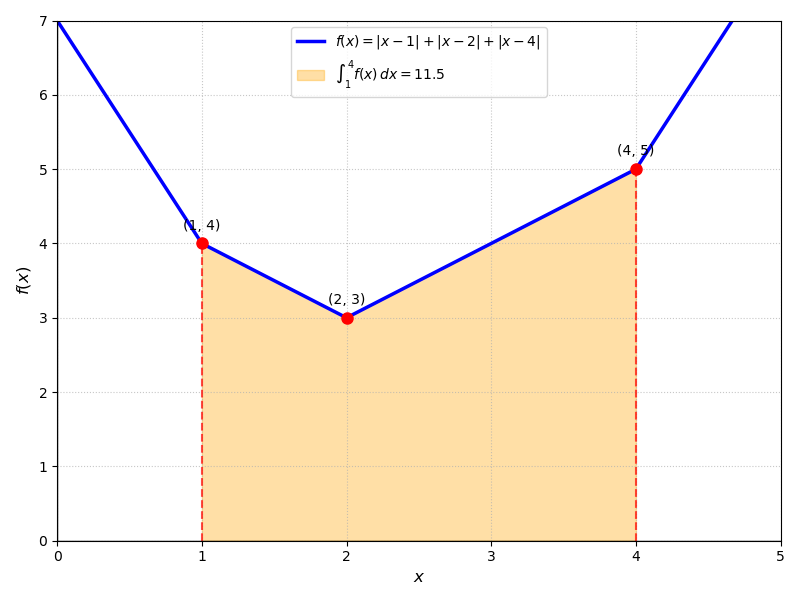
\includegraphics[width=0.75\linewidth]{figs/Integral_modulus.png}
    \caption{Integral of the modulus function}
    \label{fig:EE26BTECH11229-integral_modulus}
\end{figure}

\item 
Show that the points $A$, $B$, $C$ with position vectors $2\hat{i} - \hat{j} + \hat{k}$, $\hat{i} - 3\hat{j} - 5\hat{k}$ and $3\hat{i} - 4\hat{j} - 4\hat{k}$ respectively, are the vertices of a right-angled triangle. Hence find the area of the triangle.
\hfill (CBSE~2017)
\\
\solution
The position vectors are
\begin{align}
	\vec{A} = \myvec{2 \\ -1 \\ 1}, \quad \vec{B} = \myvec{1 \\ -3 \\ -5}, \quad \vec{C} = \myvec{3 \\ -4 \\ -4}
\end{align}
The sides are
\begin{align}
	\vec{B} - \vec{A} = \myvec{-1 \\ -2 \\ -6}, \quad \vec{C} - \vec{B} = \myvec{2 \\ -1 \\ 1}, \quad \vec{A} - \vec{C} = \myvec{-1 \\ 3 \\ 5}
\end{align}
From \eqref{eq:EE26BTECH11229-perp-vec},
\begin{align}
	\brak{\vec{B}-\vec{A}}^{\top}\brak{\vec{C}-\vec{B}} &= -2 + 2 - 6 = -6 \neq 0
	\\
	\brak{\vec{C}-\vec{B}}^{\top}\brak{\vec{A}-\vec{C}} &= -2 - 3 + 5 = 0
	\\
	\brak{\vec{A}-\vec{C}}^{\top}\brak{\vec{B}-\vec{A}} &= 1 - 6 - 30 = -35 \neq 0
\end{align}
Hence $CB \perp CA$, and the triangle is right angled at $C$. Also,
\begin{align}
	\norm{\vec{C}-\vec{B}}^2 + \norm{\vec{A}-\vec{C}}^2 = 6 + 35 = 41 = \norm{\vec{B}-\vec{A}}^2
\end{align}
From \eqref{eq:EE26BTECH11229-area-right}, the area is
\begin{align}
	A = \frac{1}{2}\sqrt{6}\sqrt{35} = \frac{\sqrt{210}}{2} \text{ sq. units}
\end{align}

The following code verifies the solution
\begin{lstlisting}[frame=single, basicstyle=\rmfamily, escapeinside={(*@}{@*)}]
(*@\makebox[\dimexpr\linewidth-2\fboxsep-2\fboxrule\relax][c]{codes/triangle.py}@*)
\end{lstlisting}
\item 
There are 4 cards numbered 1, 3, 5 and 7, one number on one card. Two cards are drawn at random without replacement. Let $X$ denote the sum of the numbers on the two drawn cards. Find the mean and variance of $X$.
\hfill (CBSE~2017)
\\
\solution
There are $6$ equally likely pairs, with sums
\begin{align}
	\brak{1,3} \to 4, \quad \brak{1,5} \to 6, \quad \brak{1,7} \to 8, \quad \brak{3,5} \to 8, \quad \brak{3,7} \to 10, \quad \brak{5,7} \to 12
\end{align}
The PMF of $X$ is
\begin{align}
	p_X\brak{4} = p_X\brak{6} = p_X\brak{10} = p_X\brak{12} = \frac{1}{6}, \quad p_X\brak{8} = \frac{2}{6} = \frac{1}{3}
\end{align}
From \eqref{eq:EE26BTECH11229-mean-var}, the mean is
\begin{align}
	E\brak{X} = \frac{4 + 6 + 2\brak{8} + 10 + 12}{6} = \frac{48}{6} = 8
\end{align}
and
\begin{align}
	\sum_{n}n^2\,p_X\brak{n} = \frac{16 + 36 + 2\brak{64} + 100 + 144}{6} = \frac{424}{6} = \frac{212}{3}
\end{align}
Therefore, the variance is
\begin{align}
	\text{Var}\brak{X} = \frac{212}{3} - 64 = \frac{20}{3}
\end{align}

The following code generates \figref{fig:EE26BTECH11229-pmf}
\begin{lstlisting}[frame=single, basicstyle=\rmfamily, escapeinside={(*@}{@*)}]
(*@\makebox[\dimexpr\linewidth-2\fboxsep-2\fboxrule\relax][c]{codes/PMF.py}@*)
\end{lstlisting}
\begin{figure}[H]
    \centering
    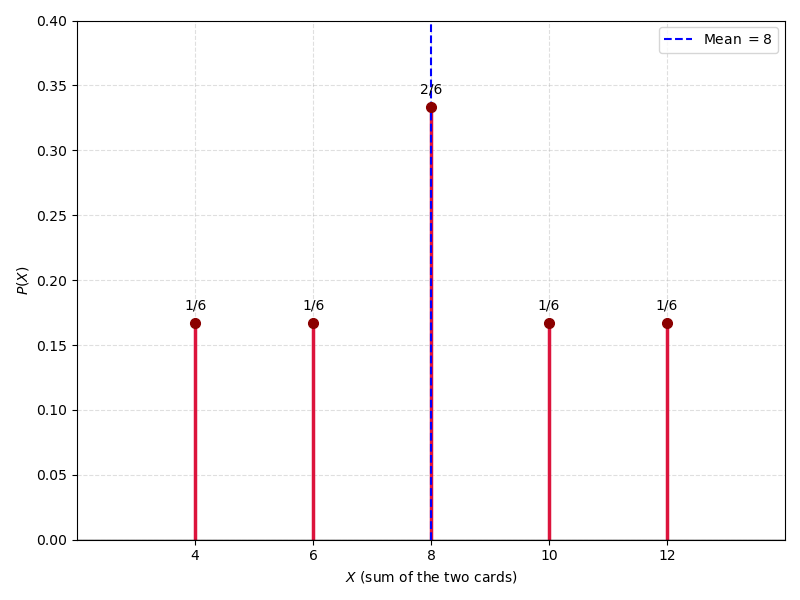
\includegraphics[width=0.75\linewidth]{figs/PMF.png}
    \caption{Probability mass function}
    \label{fig:EE26BTECH11229-pmf}
\end{figure}

\item 
Of the students in a school, it is known that 30\% have 100\% attendance and 70\% students are irregular. Previous year results report that 70\% of all students who have 100\% attendance attain A grade and 10\% irregular students attain A grade in their annual examination. At the end of the year, one student is chosen at random from the school and he was found to have an A grade. What is the probability that the student has 100\% attendance ? Is regularity required only in school ? Justify your answer.
\hfill (CBSE~2017)
\\
\solution
Let $E_1$ be the event that the student has $100\%$ attendance, $E_2$ be the event that the student is irregular and $A$ be the event that the student has an A grade. Then
\begin{align}
	\pr{E_1} = \frac{3}{10}, \quad \pr{E_2} = \frac{7}{10}, \quad \pr{A|E_1} = \frac{7}{10}, \quad \pr{A|E_2} = \frac{1}{10}
\end{align}
From \eqref{eq:EE26BTECH11229-bayes},
\begin{align}
	\pr{E_1|A} = \frac{\frac{3}{10}\cdot\frac{7}{10}}{\frac{3}{10}\cdot\frac{7}{10} + \frac{7}{10}\cdot\frac{1}{10}}
	= \frac{21}{21 + 7} = \frac{3}{4}
\end{align}
Regularity is not required only in school. It is needed in every area of life, such as studies, work, sports and health habits, because steady and regular effort gives better results. This is seen in the data above, where $70\%$ of the regular students get an A grade against $10\%$ of the irregular students.
The following code verifies the solution
\begin{lstlisting}[frame=single, basicstyle=\rmfamily, escapeinside={(*@}{@*)}]
(*@\makebox[\dimexpr\linewidth-2\fboxsep-2\fboxrule\relax][c]{codes/bayes.c}@*)
\end{lstlisting}
\item 
If $\tan^{-1}\frac{x - 3}{x - 4} + \tan^{-1}\frac{x + 3}{x + 4} = \frac{\pi}{4}$, then find the value of $x$.
\hfill (CBSE~2017)
\\
\solution
Let
\begin{align}
	a = \frac{x - 3}{x - 4}, \quad b = \frac{x + 3}{x + 4}
\end{align}
Then
\begin{align}
	a + b &= \frac{\brak{x-3}\brak{x+4} + \brak{x+3}\brak{x-4}}{x^2 - 16} = \frac{2x^2 - 24}{x^2 - 16}
	\\
	1 - ab &= \frac{\brak{x^2 - 16} - \brak{x^2 - 9}}{x^2 - 16} = \frac{-7}{x^2 - 16}
\end{align}
Taking the tangent of both sides and using \eqref{eq:EE26BTECH11229-tan-inv-sum},
\begin{align}
	\frac{a + b}{1 - ab} &= \tan\frac{\pi}{4} = 1
	\\
	\implies \frac{2x^2 - 24}{-7} &= 1
	\\
	\implies x^2 &= \frac{17}{2}
\end{align}
For this value, $ab = \frac{x^2 - 9}{x^2 - 16} = \frac{1}{15} < 1$, so \eqref{eq:EE26BTECH11229-tan-inv-sum} holds. Hence,
\begin{align}
	x = \pm\sqrt{\frac{17}{2}}
\end{align}
The following code verifies the solution
\begin{lstlisting}[frame=single, basicstyle=\rmfamily, escapeinside={(*@}{@*)}]
(*@\makebox[\dimexpr\linewidth-2\fboxsep-2\fboxrule\relax][c]{codes/root.c}@*)
\end{lstlisting}
\item 
Using properties of determinants, prove that
\begin{align*}
	\begin{vmatrix}
		a^2 + 2a & 2a + 1 & 1 \\
		2a + 1 & a + 2 & 1 \\
		3 & 3 & 1
	\end{vmatrix} = \brak{a - 1}^3
\end{align*}
\hfill (CBSE~2017)
\\
\solution
Applying $R_1 \to R_1 - R_2$ and $R_2 \to R_2 - R_3$, from \eqref{eq:EE26BTECH11229-det-props},
\begin{align}
	\begin{vmatrix}
		a^2 + 2a & 2a + 1 & 1 \\
		2a + 1 & a + 2 & 1 \\
		3 & 3 & 1
	\end{vmatrix}
	= \begin{vmatrix}
		a^2 - 1 & a - 1 & 0 \\
		2a - 2 & a - 1 & 0 \\
		3 & 3 & 1
	\end{vmatrix}
\end{align}
Expanding along the third column,
\begin{align}
	&= \begin{vmatrix}
		a^2 - 1 & a - 1 \\
		2\brak{a - 1} & a - 1
	\end{vmatrix}
	= \brak{a - 1}\brak{a - 1}\begin{vmatrix}
		a + 1 & 1 \\
		2 & 1
	\end{vmatrix}
	\\
	&= \brak{a - 1}^2\brak{a + 1 - 2} = \brak{a - 1}^3
\end{align}

The following code verifies the solution
\begin{lstlisting}[frame=single, basicstyle=\rmfamily, escapeinside={(*@}{@*)}]
(*@\makebox[\dimexpr\linewidth-2\fboxsep-2\fboxrule\relax][c]{codes/detcheck.py}@*)
\end{lstlisting}
\item 
Find matrix $\vec{A}$ such that
\begin{align*}
	\myvec{2 & -1 \\ 1 & 0 \\ -3 & 4}\vec{A} = \myvec{-1 & -8 \\ 1 & -2 \\ 9 & 22}
\end{align*}
\hfill (CBSE~2017)
\\
\solution
Let the equation be $\vec{B}\vec{A} = \vec{C}$. The columns of $\vec{A}$ satisfy $\vec{B}\vec{a}_j = \vec{c}_j$ for $j = 1, 2$, and $\vec{A}$ is a $2 \times 2$ matrix. Row reducing the augmented matrix,
\begin{align}
	\sbrak{\vec{B} \mid \vec{C}} = \myvec{2 & -1 & -1 & -8 \\ 1 & 0 & 1 & -2 \\ -3 & 4 & 9 & 22}
	\xrightarrow{R_1 \leftrightarrow R_2}
	\myvec{1 & 0 & 1 & -2 \\ 2 & -1 & -1 & -8 \\ -3 & 4 & 9 & 22}
\end{align}
\begin{align}
	\xrightarrow[R_3 \to R_3 + 3R_1]{R_2 \to R_2 - 2R_1}
	\myvec{1 & 0 & 1 & -2 \\ 0 & -1 & -3 & -4 \\ 0 & 4 & 12 & 16}
	\xrightarrow[R_2 \to -R_2]{R_3 \to R_3 + 4R_2}
	\myvec{1 & 0 & 1 & -2 \\ 0 & 1 & 3 & 4 \\ 0 & 0 & 0 & 0}
\end{align}
Here $\rank\brak{\vec{B}} = \rank\brak{\sbrak{\vec{B} \mid \vec{C}}} = 2$, which is the number of unknowns in each column. From \eqref{eq:EE26BTECH11229-consist}, the solution exists and is unique, with
\begin{align}
	\vec{a}_1 = \myvec{1 \\ 3}, \quad \vec{a}_2 = \myvec{-2 \\ 4}
\end{align}
Hence,
\begin{align}
	\vec{A} = \myvec{1 & -2 \\ 3 & 4}
\end{align}

The following code verifies the solution
\begin{lstlisting}[frame=single, basicstyle=\rmfamily, escapeinside={(*@}{@*)}]
(*@\makebox[\dimexpr\linewidth-2\fboxsep-2\fboxrule\relax][c]{codes/matrix.py}@*)
\end{lstlisting}
\item 
If $x^y + y^x = a^b$, then find $\frac{dy}{dx}$.
\hfill (CBSE~2017)
\\
\solution
Differentiating both sides with respect to $x$, and using \eqref{eq:EE26BTECH11229-log-diff},
\begin{align}
	x^y\brak{\frac{y}{x} + \ln x\,\frac{dy}{dx}} + y^x\brak{\ln y + \frac{x}{y}\frac{dy}{dx}} = 0
\end{align}
since $a^b$ is a constant. Collecting the terms in $\frac{dy}{dx}$,
\begin{align}
	\frac{dy}{dx}\brak{x^y\ln x + x\,y^{x-1}} &= -\brak{y\,x^{y-1} + y^x\ln y}
\end{align}
Therefore,
\begin{align}
	\frac{dy}{dx} = -\frac{y\,x^{y-1} + y^x\ln y}{x^y\ln x + x\,y^{x-1}}
\end{align}
\item 
Find :
\begin{align*}
	\int \frac{\sin\theta\, d\theta}{\brak{4 + \cos^2\theta}\brak{2 - \sin^2\theta}}
\end{align*}
\hfill (CBSE~2017)
\\
\solution
Substituting $t = \cos\theta$, $dt = -\sin\theta\, d\theta$ and $2 - \sin^2\theta = 1 + t^2$,
\begin{align}
	\int \frac{\sin\theta\, d\theta}{\brak{4 + \cos^2\theta}\brak{2 - \sin^2\theta}}
	= -\int \frac{dt}{\brak{4 + t^2}\brak{1 + t^2}}
\end{align}
Using partial fractions,
\begin{align}
	\frac{1}{\brak{4 + t^2}\brak{1 + t^2}} = \frac{1}{3}\sbrak{\frac{1}{1 + t^2} - \frac{1}{4 + t^2}}
\end{align}
From \eqref{eq:EE26BTECH11229-int-atan},
\begin{align}
	-\frac{1}{3}\sbrak{\tan^{-1}t - \frac{1}{2}\tan^{-1}\frac{t}{2}} + C
\end{align}
Substituting $t = \cos\theta$,
\begin{align}
	\int \frac{\sin\theta\, d\theta}{\brak{4 + \cos^2\theta}\brak{2 - \sin^2\theta}}
	= -\frac{1}{3}\tan^{-1}\brak{\cos\theta} + \frac{1}{6}\tan^{-1}\brak{\frac{\cos\theta}{2}} + C
\end{align}
\item 
Solve the following linear programming problem graphically :
\\
Maximise $Z = 34x + 45y$ under the following constraints
\begin{align*}
	x + y \le 300, \quad 2x + 3y \le 70, \quad x \ge 0, \ y \ge 0
\end{align*}
\hfill (CBSE~2017)
\\
\solution
The line $2x + 3y = 70$ meets the axes at $\brak{35, 0}$ and $\brak{0, \frac{70}{3}}$. Since $x \le 35$ and $y \le \frac{70}{3}$ in this region, $x + y \le 300$ always holds, so that constraint is redundant. The feasible region is the triangle with the corner points $\brak{0, 0}$, $\brak{35, 0}$ and $\brak{0, \frac{70}{3}}$.
From \eqref{eq:EE26BTECH11229-corner}, evaluating $Z$ at the corner points,
\begin{align}
	Z\brak{0, 0} &= 0
	\\
	Z\brak{35, 0} &= 34\brak{35} = 1190
	\\
	Z\brak{0, \tfrac{70}{3}} &= 45\brak{\tfrac{70}{3}} = 1050
\end{align}
Therefore, the maximum value of $Z$ is $1190$, at $x = 35$, $y = 0$.

The following code generates \figref{fig:EE26BTECH11229-lpp}
\begin{lstlisting}[frame=single, basicstyle=\rmfamily, escapeinside={(*@}{@*)}]
(*@\makebox[\dimexpr\linewidth-2\fboxsep-2\fboxrule\relax][c]{codes/LPP.py}@*)
\end{lstlisting}
\begin{figure}[H]
    \centering
    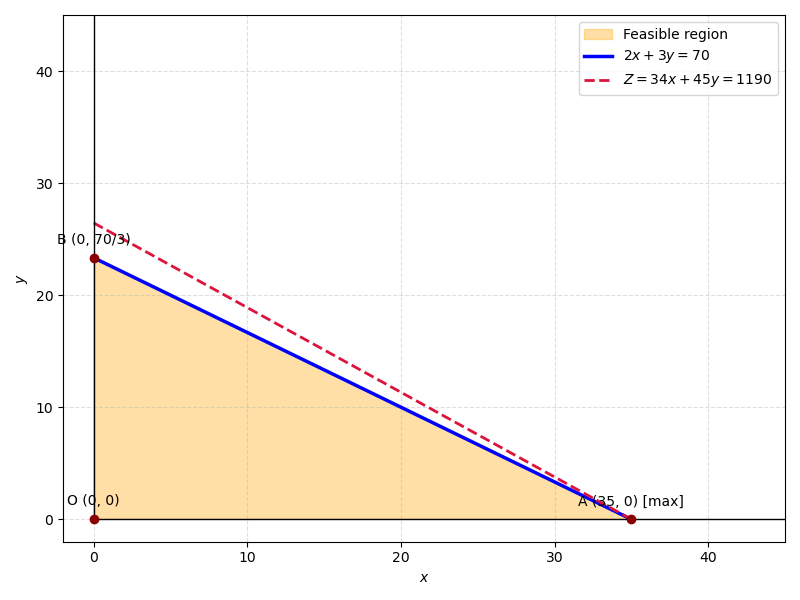
\includegraphics[width=0.75\linewidth]{figs/LPP.png}
    \caption{Linear programming problem}
    \label{fig:EE26BTECH11229-lpp}
\end{figure}

\item 
Find the value of $x$ such that the points $A\brak{3, 2, 1}$, $B\brak{4, x, 5}$, $C\brak{4, 2, -2}$ and $D\brak{6, 5, -1}$ are coplanar.
\hfill (CBSE~2017)
\\
\solution
The vectors from $\vec{A}$ are
\begin{align}
	\vec{B} - \vec{A} = \myvec{1 \\ x - 2 \\ 4}, \quad \vec{C} - \vec{A} = \myvec{1 \\ 0 \\ -3}, \quad \vec{D} - \vec{A} = \myvec{3 \\ 3 \\ -2}
\end{align}
From \eqref{eq:EE26BTECH11229-coplanar}, the points are coplanar if
\begin{align}
	\begin{vmatrix}
		1 & x - 2 & 4 \\
		1 & 0 & -3 \\
		3 & 3 & -2
	\end{vmatrix} = 0
\end{align}
Expanding along the first row,
\begin{align}
	1\brak{0 + 9} - \brak{x - 2}\brak{-2 + 9} + 4\brak{3 - 0} &= 0
	\\
	\implies 9 - 7\brak{x - 2} + 12 &= 0
	\\
	\implies 35 - 7x &= 0
	\\
	\therefore x &= 5
\end{align}
As a check, for $x = 5$, $\brak{\vec{B}-\vec{A}} + 2\brak{\vec{C}-\vec{A}} = \myvec{3 \\ 3 \\ -2} = \vec{D} - \vec{A}$, so the rank is less than $3$.

The following code verifies the solution
\begin{lstlisting}[frame=single, basicstyle=\rmfamily, escapeinside={(*@}{@*)}]
(*@\makebox[\dimexpr\linewidth-2\fboxsep-2\fboxrule\relax][c]{codes/coplanar.py}@*)
\end{lstlisting}
\item 
Find the general solution of the differential equation
\begin{align*}
	y\, dx - \brak{x + 2y^2}\, dy = 0
\end{align*}
\hfill (CBSE~2017)
\\
\solution
Rewriting the equation and multiplying by $y > 0$,
\begin{align}
	\frac{dx}{dy} - \frac{x}{y} = 2y
	\implies y\frac{dx}{dy} - x = 2y^2
	\label{eq:EE26BTECH11229-Q23-1}
\end{align}
Let $x\brak{y} \system{L} X\brak{s}$. From \eqref{eq:EE26BTECH11229-laplace-tmult} and \eqref{eq:EE26BTECH11229-laplace-deriv},
\begin{align}
	y\frac{dx}{dy} \system{L} -\frac{d}{ds}\sbrak{sX\brak{s} - x\brak{0}} = -X\brak{s} - sX^{\prime}\brak{s}
\end{align}
From \eqref{eq:EE26BTECH11229-laplace-power}, $2y^2 \system{L} \frac{4}{s^3}$. Taking the Laplace transform of \eqref{eq:EE26BTECH11229-Q23-1},
\begin{align}
	-X - sX^{\prime} - X &= \frac{4}{s^3}
	\\
	\implies X^{\prime} + \frac{2}{s}X &= -\frac{4}{s^4}
\end{align}
Multiplying by $s^2$,
\begin{align}
	\frac{d}{ds}\brak{s^2X} &= -\frac{4}{s^2}
	\\
	\implies s^2X &= \frac{4}{s} + C
	\\
	\implies X\brak{s} &= \frac{4}{s^3} + \frac{C}{s^2}
\end{align}
Taking the inverse Laplace transform using \eqref{eq:EE26BTECH11229-laplace-power},
\begin{align}
	x\brak{y} = 2y^2 + Cy
\end{align}
Note that $x\brak{0}$ cancelled out, so $C$ remains arbitrary. As a check, $\frac{dx}{dy} = 4y + C$ and $\frac{x}{y} + 2y = 2y + C + 2y = 4y + C$. Therefore, the general solution is
\begin{align}
	x = 2y^2 + Cy
\end{align}
\item 
Find the coordinates of the point where the line through the points $\brak{3, -4, -5}$ and $\brak{2, -3, 1}$, crosses the plane determined by the points $\brak{1, 2, 3}$, $\brak{4, 2, -3}$ and $\brak{0, 4, 3}$.
\hfill (CBSE~2017)
\\
\solution
Let $\vec{A} = \myvec{1 \\ 2 \\ 3}$, $\vec{B} = \myvec{4 \\ 2 \\ -3}$, $\vec{C} = \myvec{0 \\ 4 \\ 3}$. Then
\begin{align}
	\vec{B} - \vec{A} = \myvec{3 \\ 0 \\ -6}, \quad \vec{C} - \vec{A} = \myvec{-1 \\ 2 \\ 0}
\end{align}
From \eqref{eq:EE26BTECH11229-plane-3pts}, a normal to the plane is
\begin{align}
	\vec{n} = \myvec{3 \\ 0 \\ -6}\times\myvec{-1 \\ 2 \\ 0} = \myvec{12 \\ 6 \\ 6} \propto \myvec{2 \\ 1 \\ 1}
\end{align}
and the plane is
\begin{align}
	\myvec{2 & 1 & 1}\vec{x} = 2 + 2 + 3 = 7
\end{align}
The line through $\vec{P} = \myvec{3 \\ -4 \\ -5}$ and $\vec{Q} = \myvec{2 \\ -3 \\ 1}$ has the direction $\vec{m} = \vec{Q} - \vec{P} = \myvec{-1 \\ 1 \\ 6}$. From \eqref{eq:EE26BTECH11229-line-param},
\begin{align}
	\vec{x} = \myvec{3 \\ -4 \\ -5} + \kappa\myvec{-1 \\ 1 \\ 6}
\end{align}
Substituting in the equation of the plane,
\begin{align}
	\brak{-3} + 5\kappa &= 7
	\\
	\implies \kappa &= 2
\end{align}
Therefore, the point of intersection is
\begin{align}
	\vec{x} = \myvec{3 \\ -4 \\ -5} + 2\myvec{-1 \\ 1 \\ 6} = \myvec{1 \\ -2 \\ 7}
\end{align}

The following code verifies the solution
\begin{lstlisting}[frame=single, basicstyle=\rmfamily, escapeinside={(*@}{@*)}]
(*@\makebox[\dimexpr\linewidth-2\fboxsep-2\fboxrule\relax][c]{codes/lineplane.py}@*)
\end{lstlisting}
\item 
Find the particular solution of the differential equation $\brak{x - y}\frac{dy}{dx} = \brak{x + 2y}$, given that $y = 0$ when $x = 1$.
\hfill (CBSE~2017)
\\
\solution
The equation contains the product $y\frac{dy}{dx}$, so it cannot be transformed directly. Introducing a parameter $t$ such that
\begin{align}
	\frac{dx}{dt} = x - y, \quad \frac{dy}{dt} = x + 2y
\end{align}
gives $\frac{dy}{dx} = \frac{dy/dt}{dx/dt} = \frac{x + 2y}{x - y}$, which is the given equation. In matrix form,
\begin{align}
	\frac{d}{dt}\myvec{x \\ y} = \myvec{1 & -1 \\ 1 & 2}\myvec{x \\ y}, \quad \myvec{x \\ y}_{t = 0} = \myvec{1 \\ 0}
\end{align}
Let $\vec{M} = \myvec{1 & -1 \\ 1 & 2}$. Then $\text{tr}\brak{\vec{M}} = 3$ and $\mydet{\vec{M}} = 3$. From \eqref{eq:EE26BTECH11229-char-poly},
\begin{align}
	\mydet{s\vec{I} - \vec{M}} = s^2 - 3s + 3 = \brak{s - \frac{3}{2}}^2 + \brak{\frac{\sqrt{3}}{2}}^2
\end{align}
so the eigenvalues are $\frac{3 \pm j\sqrt{3}}{2}$. From \eqref{eq:EE26BTECH11229-laplace-system},
\begin{align}
	\myvec{X\brak{s} \\ Y\brak{s}} = \myvec{s - 1 & 1 \\ -1 & s - 2}^{-1}\myvec{1 \\ 0}
	= \frac{1}{s^2 - 3s + 3}\myvec{s - 2 \\ 1}
\end{align}
Writing $s - 2 = \brak{s - \frac{3}{2}} - \frac{1}{2}$,
\begin{align}
	X\brak{s} &= \frac{s - \frac{3}{2}}{\brak{s - \frac{3}{2}}^2 + \frac{3}{4}} - \frac{1}{\sqrt{3}}\cdot\frac{\frac{\sqrt{3}}{2}}{\brak{s - \frac{3}{2}}^2 + \frac{3}{4}}
	\\
	Y\brak{s} &= \frac{2}{\sqrt{3}}\cdot\frac{\frac{\sqrt{3}}{2}}{\brak{s - \frac{3}{2}}^2 + \frac{3}{4}}
\end{align}
Taking the inverse Laplace transform using \eqref{eq:EE26BTECH11229-laplace-shift} and \eqref{eq:EE26BTECH11229-laplace-sincos}, with $\theta = \frac{\sqrt{3}}{2}t$,
\begin{align}
	x\brak{t} &= e^{\frac{3t}{2}}\brak{\cos\theta - \frac{1}{\sqrt{3}}\sin\theta}
	\\
	y\brak{t} &= \frac{2}{\sqrt{3}}e^{\frac{3t}{2}}\sin\theta
\end{align}
To eliminate $t$,
\begin{align}
	x + 2y &= 2e^{\frac{3t}{2}}\sin\brak{\theta + \frac{\pi}{6}}, \quad \sqrt{3}x = 2e^{\frac{3t}{2}}\cos\brak{\theta + \frac{\pi}{6}}
	\\
	\implies \frac{x + 2y}{\sqrt{3}x} &= \tan\brak{\theta + \frac{\pi}{6}}
	\\
	\implies \tan^{-1}\brak{\frac{x + 2y}{\sqrt{3}x}} &= \frac{\sqrt{3}}{2}t + \frac{\pi}{6}
\end{align}
Also, since $x + \frac{y}{2} = e^{\frac{3t}{2}}\cos\theta$,
\begin{align}
	x^2 + xy + y^2 = \brak{x + \frac{y}{2}}^2 + \frac{3}{4}y^2 = e^{3t}\brak{\cos^2\theta + \sin^2\theta} = e^{3t}
	\\
	\implies \frac{1}{2}\ln\brak{x^2 + xy + y^2} = \frac{3t}{2}
\end{align}
Eliminating $t$ from the last two results, the particular solution is
\begin{align}
	\sqrt{3}\tan^{-1}\brak{\frac{x + 2y}{\sqrt{3}x}} - \frac{1}{2}\ln\brak{x^2 + xy + y^2} = \frac{\pi}{2\sqrt{3}}
\end{align}
which holds on the branch through $\brak{1, 0}$. As a check, at $\brak{1, 0}$ the left side is $\sqrt{3}\cdot\frac{\pi}{6} - 0 = \frac{\pi}{2\sqrt{3}}$.

The following code generates \figref{fig:EE26BTECH11229-euler}
\begin{lstlisting}[frame=single, basicstyle=\rmfamily, escapeinside={(*@}{@*)}]
(*@\makebox[\dimexpr\linewidth-2\fboxsep-2\fboxrule\relax][c]{codes/euler.py}@*)
\end{lstlisting}
\begin{figure}[H]
    \centering
    \includegraphics[width=0.75\linewidth]{figs/euler.png}
    \caption{Euler's method}
    \label{fig:EE26BTECH11229-euler}
\end{figure}
\item
Find the area enclosed between the parabola $4y = 3x^2$ and the straight line $3x - 2y + 12 = 0$.
\hfill (CBSE~2017)
\\
\solution
The parabola $3x^2 - 4y = 0$ is a conic with
\begin{align}
	\vec{V} = \myvec{3 & 0 \\ 0 & 0}, \quad \vec{u} = \myvec{0 \\ -2}, \quad f = 0
\end{align}
The line $3x - 2y + 12 = 0$ is $\vec{x} = \vec{h} + \kappa\vec{m}$ with
\begin{align}
	\vec{h} = \myvec{0 \\ 6}, \quad \vec{m} = \myvec{2 \\ 3}
\end{align}
Then
\begin{align}
	\vec{V}\vec{h} + \vec{u} = \myvec{0 \\ -2}, \quad \vec{m}^{\top}\brak{\vec{V}\vec{h} + \vec{u}} = -6, \quad g\brak{\vec{h}} = -24, \quad \vec{m}^{\top}\vec{V}\vec{m} = 12
\end{align}
From \eqref{eq:EE26BTECH11229-line-conic},
\begin{align}
	\kappa = \frac{6 \pm \sqrt{36 + 288}}{12} = \frac{6 \pm 18}{12} = 2 \text{ or } -1
\end{align}
The points of intersection are
\begin{align}
	\myvec{0 \\ 6} + 2\myvec{2 \\ 3} = \myvec{4 \\ 12}, \quad \myvec{0 \\ 6} - \myvec{2 \\ 3} = \myvec{-2 \\ 3}
\end{align}
The line is above the parabola between $x = -2$ and $x = 4$. From \eqref{eq:EE26BTECH11229-area-curves},
\begin{align}
	A &= \int_{-2}^{4}\sbrak{\frac{3x + 12}{2} - \frac{3x^2}{4}}\, dx
	= \sbrak{\frac{3x^2}{4} + 6x - \frac{x^3}{4}}_{-2}^{4}
	\\
	&= 20 - \brak{-7} = 27 \text{ sq. units}
\end{align}

The following code generates \figref{fig:EE26BTECH11229-parabola_line}
\begin{lstlisting}[frame=single, basicstyle=\rmfamily, escapeinside={(*@}{@*)}]
(*@\makebox[\dimexpr\linewidth-2\fboxsep-2\fboxrule\relax][c]{codes/parabola\_line.py}@*)
\end{lstlisting}
\begin{figure}[H]
    \centering
    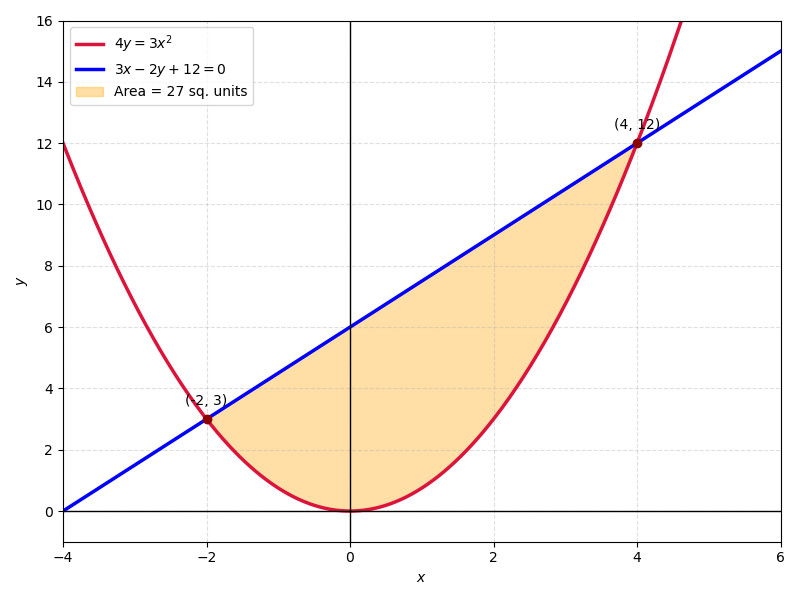
\includegraphics[width=0.75\linewidth]{figs/parabola_line.png}
    \caption{Parabola and line}
    \label{fig:EE26BTECH11229-parabola_line}
\end{figure}

\item 
Consider $f: \mathbb{R} - \cbrak{-\frac{4}{3}} \to \mathbb{R} - \cbrak{\frac{4}{3}}$ given by $f\brak{x} = \frac{4x + 3}{3x + 4}$. Show that $f$ is bijective. Find the inverse of $f$ and hence find $f^{-1}\brak{0}$ and $x$ such that $f^{-1}\brak{x} = 2$.
\hfill (CBSE~2017)
\\
\solution
From \eqref{eq:EE26BTECH11229-bij}, for one-one,
\begin{align}
	f\brak{x_1} = f\brak{x_2} &\implies \brak{4x_1 + 3}\brak{3x_2 + 4} = \brak{4x_2 + 3}\brak{3x_1 + 4}
	\\
	&\implies 7x_1 = 7x_2 \implies x_1 = x_2
\end{align}
For onto, let $y = \frac{4x + 3}{3x + 4}$ with $y \neq \frac{4}{3}$. Solving for $x$,
\begin{align}
	x = \frac{3 - 4y}{3y - 4}
\end{align}
which is defined for every $y \neq \frac{4}{3}$, and $x \neq -\frac{4}{3}$, since $x = -\frac{4}{3}$ would give $-9 = -16$. So $f$ is onto and hence bijective. The inverse is
\begin{align}
	f^{-1}\brak{x} = \frac{3 - 4x}{3x - 4}
\end{align}
From \eqref{eq:EE26BTECH11229-mobius}, $\vec{M} = \myvec{4 & 3 \\ 3 & 4}$ with $\mydet{\vec{M}} = 7 \neq 0$, and $\vec{M}^{-1} = \frac{1}{7}\myvec{4 & -3 \\ -3 & 4}$ gives the same inverse $\frac{4x - 3}{-3x + 4}$. Then
\begin{align}
	f^{-1}\brak{0} = \frac{3}{-4} = -\frac{3}{4}
\end{align}
and
\begin{align}
	f^{-1}\brak{x} = 2 \implies 3 - 4x = 6x - 8 \implies x = \frac{11}{10}
\end{align}
\item 
Let $A = \mathbb{Q} \times \mathbb{Q}$ and let $*$ be a binary operation on $A$ defined by $\brak{a, b} * \brak{c, d} = \brak{ac, b + ad}$ for $\brak{a, b}, \brak{c, d} \in A$. Determine, whether $*$ is commutative and associative. Then, with respect to $*$ on $A$
\begin{enumerate}
	\item Find the identity element in $A$.
	\item Find the invertible elements of $A$.
\end{enumerate}
\hfill (CBSE~2017)
\\
\solution
Writing $\brak{a, b}$ as the matrix $\myvec{a & b \\ 0 & 1}$, the product
\begin{align}
	\myvec{a & b \\ 0 & 1}\myvec{c & d \\ 0 & 1} = \myvec{ac & ad + b \\ 0 & 1}
\end{align}
is exactly $\brak{a, b} * \brak{c, d}$.
\begin{enumerate}
\item \textbf{Commutative:} $\brak{a, b} * \brak{c, d} = \brak{ac, b + ad}$ whereas $\brak{c, d} * \brak{a, b} = \brak{ac, d + cb}$. For $\brak{1, 2} * \brak{3, 4} = \brak{3, 6}$ and $\brak{3, 4} * \brak{1, 2} = \brak{3, 10}$. So $*$ is not commutative.
\item \textbf{Associative:}
\begin{align}
	\sbrak{\brak{a, b} * \brak{c, d}} * \brak{e, f} &= \brak{ac, b + ad} * \brak{e, f} = \brak{ace, b + ad + acf}
	\\
	\brak{a, b} * \sbrak{\brak{c, d} * \brak{e, f}} &= \brak{a, b} * \brak{ce, d + cf} = \brak{ace, b + ad + acf}
\end{align}
The two are equal, so $*$ is associative.
\item \textbf{Identity:} Let $\brak{e_1, e_2}$ be the identity. Then $\brak{a, b} * \brak{e_1, e_2} = \brak{ae_1, b + ae_2} = \brak{a, b}$ for all $a, b$, giving $e_1 = 1$, $e_2 = 0$. The identity element is $\brak{1, 0}$, which also satisfies $\brak{1, 0} * \brak{a, b} = \brak{a, b}$.
\item \textbf{Invertible elements:} For $\brak{c, d}$ to be the inverse of $\brak{a, b}$,
\begin{align}
	\brak{ac, b + ad} = \brak{1, 0} \implies c = \frac{1}{a}, \quad d = -\frac{b}{a}
\end{align}
which requires $a \neq 0$. So the invertible elements are $\brak{a, b}$ with $a \neq 0$, and the inverse is $\brak{\frac{1}{a}, -\frac{b}{a}}$. In matrix form, this is $\mydet{\myvec{a & b \\ 0 & 1}} = a \neq 0$.
\end{enumerate}
\item 
If $\vec{A} = \myvec{2 & -3 & 5 \\ 3 & 2 & -4 \\ 1 & 1 & -2}$, find $\vec{A}^{-1}$. Hence using $\vec{A}^{-1}$ solve the system of equations $2x - 3y + 5z = 11$, $3x + 2y - 4z = -5$, $x + y - 2z = -3$.
\hfill (CBSE~2017)
\\
\solution
The determinant of $\vec{A}$ is
\begin{align}
	\mydet{\vec{A}} = 2\brak{-4 + 4} + 3\brak{-6 + 4} + 5\brak{3 - 2} = 0 - 6 + 5 = -1 \neq 0
\end{align}
The cofactors are
\begin{align}
	C_{11} = 0, \ C_{12} = 2, \ C_{13} = 1, \ C_{21} = -1, \ C_{22} = -9, \ C_{23} = -5, \ C_{31} = 2, \ C_{32} = 23, \ C_{33} = 13
\end{align}
so
\begin{align}
	\text{adj}\brak{\vec{A}} = \myvec{0 & -1 & 2 \\ 2 & -9 & 23 \\ 1 & -5 & 13}
\end{align}
From \eqref{eq:EE26BTECH11229-inverse},
\begin{align}
	\vec{A}^{-1} = \frac{1}{-1}\myvec{0 & -1 & 2 \\ 2 & -9 & 23 \\ 1 & -5 & 13} = \myvec{0 & 1 & -2 \\ -2 & 9 & -23 \\ -1 & 5 & -13}
\end{align}
The system is $\vec{A}\vec{x} = \vec{b}$ with $\vec{x} = \myvec{x \\ y \\ z}$ and $\vec{b} = \myvec{11 \\ -5 \\ -3}$. Since $\rank\brak{\vec{A}} = \rank\brak{\sbrak{\vec{A} \mid \vec{b}}} = 3$, from \eqref{eq:EE26BTECH11229-consist} the solution is unique. From \eqref{eq:EE26BTECH11229-inverse},
\begin{align}
	\vec{x} = \vec{A}^{-1}\vec{b} = \myvec{0 & 1 & -2 \\ -2 & 9 & -23 \\ -1 & 5 & -13}\myvec{11 \\ -5 \\ -3} = \myvec{1 \\ 2 \\ 3}
\end{align}
Therefore,
\begin{align}
	x = 1, \quad y = 2, \quad z = 3
\end{align}

The following code verifies the solution
\begin{lstlisting}[frame=single, basicstyle=\rmfamily, escapeinside={(*@}{@*)}]
(*@\makebox[\dimexpr\linewidth-2\fboxsep-2\fboxrule\relax][c]{codes/inverse.py}@*)
\end{lstlisting}
\end{enumerate}
